 
\chapter{中介分析：自然直接效应与间接效应}
 \label{chapter::mediation}




设处理中间变量$M$位于处理$Z$与结果$Y$之间。按$U = \{  M(1), M(0) \}$定义的主层内因果效应，可以评价潜在亚组$U$间的处理效应异质性。若$M$确实位于$Z$到$Y$的因果路径上，主层效应$\tau(1,1)$和$ \tau(0,0)$可提供$Z$对$Y$直接效应的信息，但仅针对这两个潜在亚组。另两个主层效应$\tau(1,0)$和$ \tau(0,1)$则同时包含直接与间接效应。从根本上说，主分层甚至不假定$M$可被干预，因此不能提供$Z$经由$M$影响$Y$的间接效应的信息。 



前文讨论中，我以非严谨的方式使用了“直接效应”与“间接效应”这两个术语。当 $M$ 确属从 $Z$ 指向 $Y$ 的因果途径时，研究者常希望探明 $Z$ 对 $Y$ 的效应有多少经由 $M$ 产生、多少经由其他路径实现。此类分析即被称为{\it 中介分析}，也是本章的主题。 



\section{示例说明}





进行中介分析时需考虑以下变量：处理因素 $Z$、结果变量 $Y$、中介变量 $M$ 以及若干协变量 $X$。图 \ref{fg::mediationDAG} 展示了这些变量间的关系。下面列举几个具体实例。 



\begin{figure}[ht]
\centering
$$
\begin{xy}
\xymatrix{
&& X \ar[dll] \ar[d] \ar[drr] \\
Z \ar[rr] \ar@/_1.5pc/[rrrr] & & M\ar[rr] & & Y}
\end{xy}
$$
\caption{中介分析的因果示意图}\label{fg::mediationDAG}
\end{figure}


\begin{example}
\citet{Vanderweele::2012genetic}通过中介分析，研究染色体 15q25.1 上的遗传变异对肺癌的效应，有多少经由吸烟传递、有多少通过其他因果路径产生。\footnote{回顾第\ref{chapter::evalue}章 Fisher 关于共同遗传因素同时影响吸烟与肺癌的假说。}暴露水平对应 C 等位基因数从 0 变为 2；吸烟强度用每日吸烟支数的平方根衡量；结果是肺癌指标。\citet{Vanderweele::2012genetic}的研究还包含许多社会人口学协变量。  %case-control
\end{example}



\begin{example}
\citet{rudolph2018causal} 研究了社区贫困状况如何通过学校环境及同伴网络间接影响青少年的药物滥用问题。数据源自2001至2004年间对美国青少年开展的全国性代表性调查——共病调查复制青少年补充研究。处理因素定义为居住地是否属于美国人口普查所确定的社会经济地位最低区域，并以二元变量表示。四个二元变量衡量学校环境及同伴关系；六个二元变量则用于评估药物使用情况。其他控制因素包括性别、年龄、种族、移民代际、家庭收入等特征。
\end{example}


\begin{example}\label{eg::mediation-jobs}
\ri{R}的\ri{mediation}包包含\ri{jobs}数据，来自 JOBS II 随机实地实验，用于评价职业培训干预对失业者的成效。第\ref{sec::cace-application}节使用过该数据。项目不仅旨在促进失业者再就业，也希望改善求职者心理健康。因此，需要评价干预通过求职自我效能感影响心理健康的间接效应，以及通过其他路径产生的直接效应。后文第\ref{section::BK-jobs}节将重新分析此例。 
\end{example}



\section{嵌套潜在结果模型}


\subsection{自然直接效应与自然间接效应}下面省略单位$i$的下标$i$，假定所有随机变量都是从超总体独立同分布抽取的。为简化讨论，着重考虑二元处理$Z$。 

 
先考虑对$z$的假想干预，并定义对应于干预$z$的潜在中介与结果：
$$
\{ M(z) , Y(z): z=0,1\}.
$$
再考虑同时干预$z$和$m$，定义对应于$z$与$m$的潜在结果：
$$
\{ Y(z, m): z=0, 1; m \in \mathcal{M}  \},
$$
其中$ \mathcal{M} $包含$m$的全部可能取值。\citet{Robins::1992}和\citet{Pearl::2001}进一步考虑对$z$及$m = M(z')  $干预对应的嵌套潜在结果：
$$
\{ Y(z, M_{z'}) : z = 0,1; z'=0,1   \}
$$
为避免括号过多，将$M(z')$写成$ M_{z'}$。$Y(z, M_{z'})$表示：若将处理设为$z$，同时将中介设为处理$z'$下的潜在取值$M(z')$，将会出现的假想结果。$z$与$z'$可以不同。二元处理共有四个嵌套潜在结果：
$$
\{ Y( 1, M_1),    Y( 1, M_0),  Y( 0, M_1),  Y( 0, M_0) \}.
$$
$Y(1, M_1)$表示将处理设为$z=1$，中介取其在$z=1$下自然会出现的值时的结果；类似地，$Y(0, M_0)$表示处理为$z=0$、中介取其在$z=0$下自然值时的结果。若$Y(1, M_1) \neq  Y(1)$或$Y(0, M_0) \neq  Y(0)$，就很不自然。因此，本章始终采用以下合成假设。

\begin{assumption}
[合成假设]\label{assume::composition}
对任意 $z=0,1$，均满足 $Y(z, M_z) =   Y(z)$。 
\end{assumption}


合成假设无法证明，它确实是一项假设。也可以直接将$Y(1)$定义为$Y(1, M_1)$、将$ Y(0)$定义为$Y(0, M_0) $，从而避免哲学争论。这样，假设\ref{assume::composition}按定义成立。 



$Y(1,M_0)$表示单位接受处理$1$，但中介被设为未处理时自然值$M_0$的假想结果。类似地，$Y(0,M_1)$表示单位接受对照$0$，但中介被设为处理时自然值$M_1$的假想结果。这是两个跨世界反事实项，可用来定义直接与间接效应。 


\begin{definition}
[总效应、直接效应与间接效应]
\label{def::mediation}
将处理对结果的整体效应定义为
$$
\tau = E\{ Y(1)  - Y(0) \}.
$$
自然直接效应定义为
$$
\NDE = E\{  Y(1,M_0) - Y(0, M_0)  \}. 
$$
自然间接效应定义为 
$$
\NIE = E\{  Y(1, M_1) - Y(1, M_0) \} .
$$
\end{definition}


总效应就是$Z$对$Y$的通常平均因果效应。自然直接效应衡量将中介固定在无干预时自然值$M_0$后，处理对结果的效应；自然间接效应则将处理本身固定为$z=1$，衡量改变中介所传递的处理效应。在合成假设下，二者简化为
$$
\NDE = E\{  Y(1,M_0) - Y(0)  \} ,\quad
\NIE = E\{  Y(1) - Y(1, M_0) \},
$$
因此，总效应可分解为自然直接效应与自然间接效应之和。


\begin{proposition}
\label{prop::mediation-decomposition}
依据定义 \ref{def::mediation}与假设 \ref{assume::composition}，即有
$$
\tau = \NDE + \NIE .
$$
\end{proposition}

数学上，也可将自然间接效应定义为$ E\{  Y(0, M_1) - Y(0, M_0) \}$，此时处理固定为$0$。但这一替代定义不能与前述自然直接效应一起得到命题\ref{prop::mediation-decomposition}的分解。 

遗憾的是，嵌套潜在结果$Y(1,M_0)$涉及跨世界干预，难以理解：处理设为$z=1$，中介却取处理$z=0$下的自然值$M_0$。这两种处理干预显然不能在同一次实际实验中同时发生。为理解$Y(1,M_0)$，需要设想图\ref{fg::crossworld}那样的平行世界。以$Y(1,M_0)$为例：处理设为$z=1$时，中介必取$M_1$；若同时要求中介为$m=M_0$，就需要从平行世界的另一场实验中，得知同一单位的$M_0$。这在真实物理实验中可能无法实现，因为需要同一单位同时接受两个不同处理水平。若对单位同质性作较强假设，或许能用另一单位在对照状态下的中介值作为$M_0$的替代。 



 
\subsection{形而上学还是科学？}
\label{sec::popper-science}

因果推断极为复杂，连基本符号系统也尚无共识。\citet{Robins::1992}与\citet{Pearl::2001}利用嵌套潜在结果描述直接与间接效应。但\citet{frangakis2002principal}认为 $Y(1,M_0)$ 与 $Y(0, M_1)$ 属于无法被实验观测到的{\it 先验反事实值}，因而带有形而上学色彩。依据\citet{popper1963conjectures}的学说：一个命题若无法通过任何实验证伪则属形而上学范畴。由于 $Y(1,M_0)$ 和 $Y(0, M_1)$ 均无法观测，除极其有限的平凡命题外我们无法验证任何与之相关的论断，因此纯粹的贝叶斯统计学家可能视中介分析为某种形而上学研究。 


更进一步，\citet{dawid2000causal}批评潜在结果框架具有形而上学性质，将第\ref{sec::po-sciencetable}章 Rubin 的“科学表”称为“形而上学数组”。他的批评不仅针对$Y(1,M_0)$与$Y(0, M_1)$这些先验反事实，也针对更简单的$Y(1)$与$Y(0)$。\citet{dawid2000causal}认为，既然$Y(1)$与$Y(0)$永远不能同时观测，引入$\{ Y(1), Y(0)\}$就是形而上学活动。对联合分布$\pr\{ Y(1) , Y(0) \}$的不可观测性，他的看法有道理；对边际分布却并非如此。观测数据确实能证伪有关边际分布的一些命题，尽管无法一般地检验联合分布的具体依赖结构。\footnote{根据概率论，给定边际分布$\pr( Y(1) \leq y_1 ) $与$\pr( Y(0) \leq y_0 ) $，Fréchet--Hoeffding 不等式可约束联合分布$\pr( Y(1) \leq y_1 , Y(0) \leq y_0 ) $：
\begin{eqnarray*}
&&\max\{  0,  \pr( Y(1) \leq y_1) +\pr( Y(0) \leq y_0 ) - 1  \}  \\
&\leq& 
\pr( Y(1) \leq y_1 , Y(0) \leq y_0 ) \\
&\leq& 
\min\{ \pr( Y(1) \leq y_1) , \pr( Y(0) \leq y_0 )  \}.
\end{eqnarray*}
该界往往很宽松；不加额外假设，就没有超出此不等式的更多信息。}因此，即使按\citet{popper1963conjectures}的标准，Rubin 的科学表也不能整体视为形而上学，因为它有非平凡的可证伪推论，虽然并非所有推论都可证伪。这正是$\{ Y(1), Y(0)\}$与$\{ Y(1,M_0), Y(0, M_1) \} $的根本区别。
 


\begin{figure}[ht]
\centering
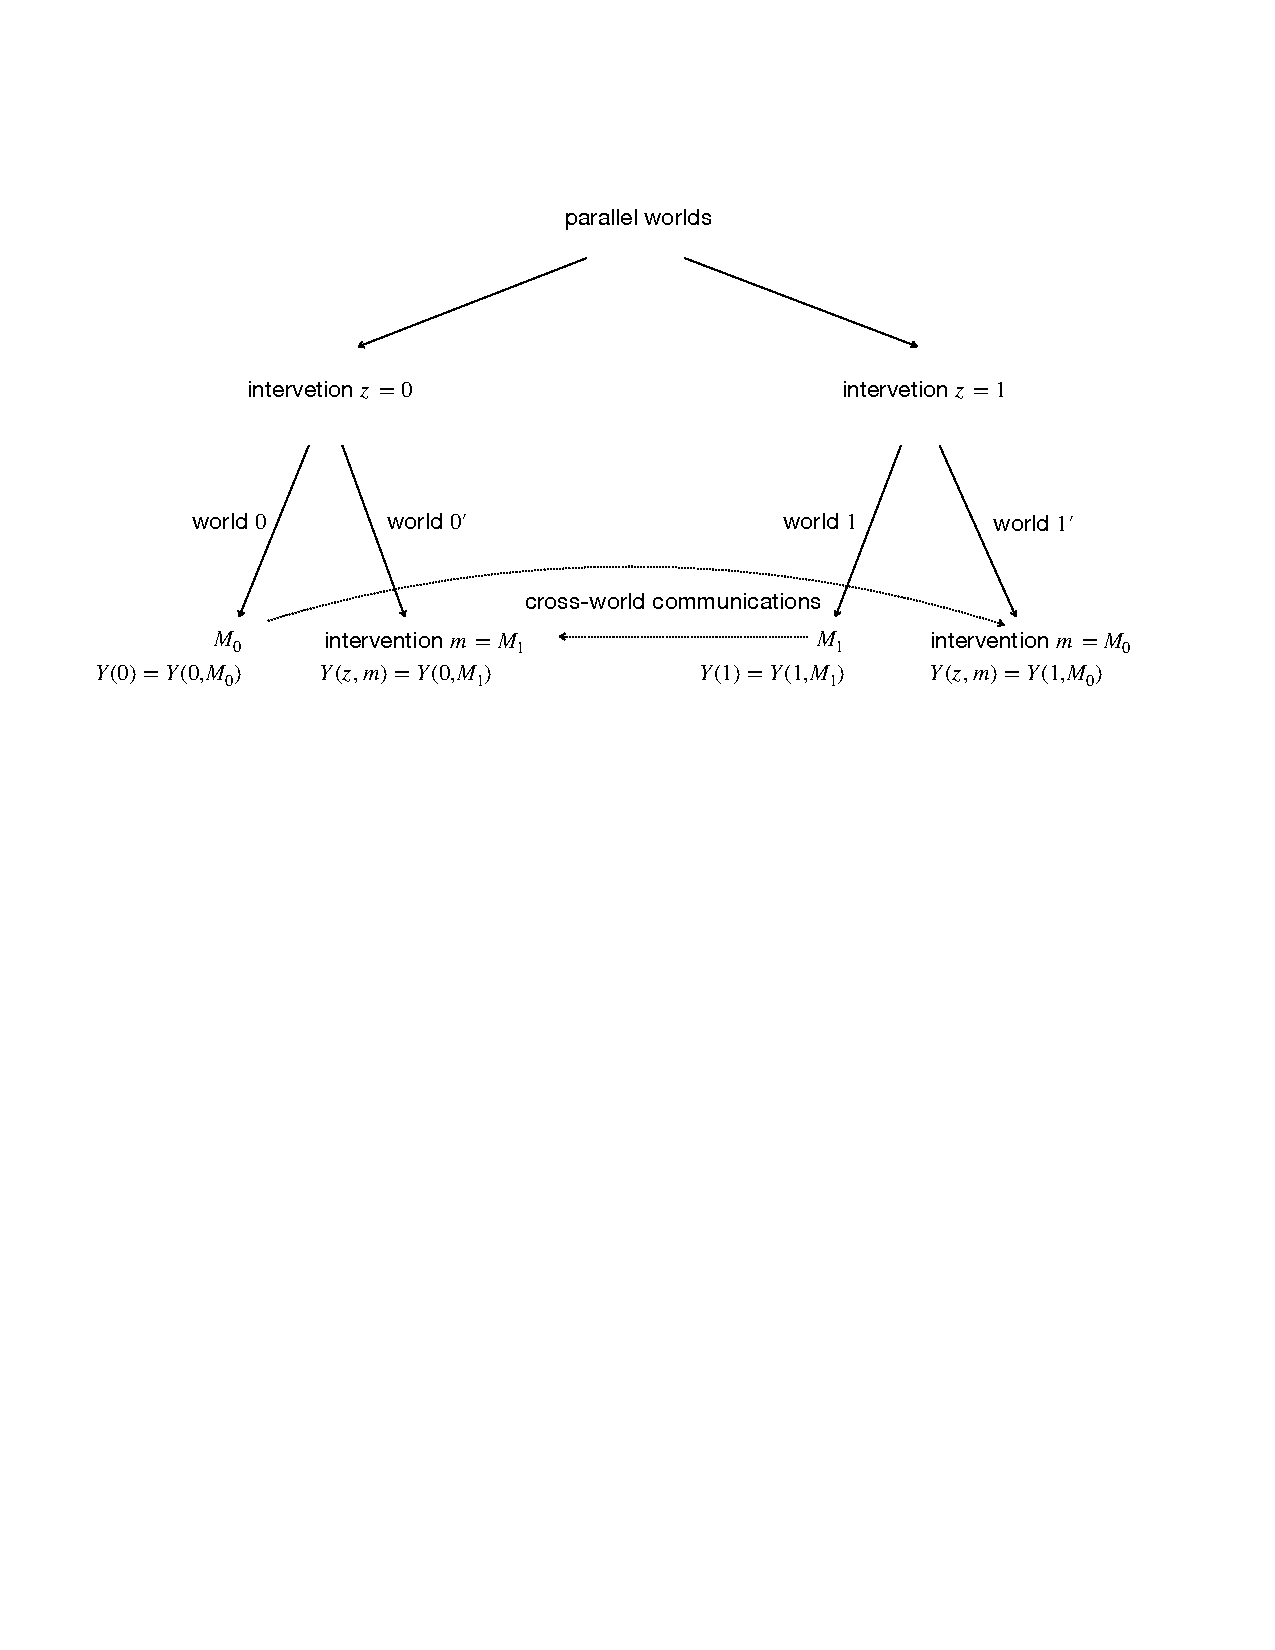
\includegraphics[width =  \textwidth]{figures/crossworld.pdf}
\caption{跨情境潜在结果 $Y(1,M_0)$ 与 $Y(0, M_1)$ 的概念示意图}\label{fg::crossworld}
\end{figure}




\section{中介效应计算公式}

\citet{Pearl::2001}的中介公式推导基于下述四重假设。前三重假设实质要求处理与中介均需在给定协变量条件下呈随机化分布。

\begin{assumption}
\label{assume::mediation1}
不存在处理与结果之间的混杂：
$$
Z\ind Y(z,m)\mid X
$$
对所有$z$与$m$成立。
\end{assumption}

\begin{assumption}
\label{assume::mediation2}
不存在中介与结果之间的混杂：
$$
M \ind Y(z,m) \mid (X, Z)
$$
对所有$z$与$m$成立。
\end{assumption}

假设\ref{assume::mediation1}与\ref{assume::mediation2}合称{\it 序贯可忽略性}，等价于给定$X$后$(Z, M)$联合随机化：
\begin{eqnarray}\label{eq::joint-randomization}
(Z, M) \ind Y(z,m)\mid X
\end{eqnarray}
对所有$z$与$m$成立。\eqref{eq::joint-randomization}的证明留作习题\ref{para::sr-jr}。 



\begin{assumption}
\label{assume::mediation3}
处理与中介间无混杂效应：
$$
Z \ind M(z) \mid X
$$ 
对所有可能值 $z$ 均成立。 
\end{assumption}

最后第四重假设涉及跨情境独立性： 

\begin{assumption}
\label{assume::mediation4}
不存在跨情境独立性：
$$
Y(z,m) \ind M(z') \mid X
$$ 
对所有可能值 $z,z'$ 与 $m$ 均成立。 
\end{assumption}


假设\ref{assume::mediation1}至\ref{assume::mediation3}很强，但至少在处理与中介均随机化的实验中成立。假设\ref{assume::mediation4}更强，没有物理实验能够保证它。$z\neq z'$时，任何实验都不能同时观测$Y(z,m)$与$ M(z') $，因此假设\ref{assume::mediation4}永远无法验证，具有根本的形而上学性质。 

下面给出假设\ref{assume::mediation1}至\ref{assume::mediation4}全部成立的例子。 

\begin{example}
\label{eg::mediation-assumptions}
给定$X$，生成
\begin{eqnarray*}
Z &=& 1\{  g_Z(X, \varepsilon_Z)  \geq 0 \} ,\\
M(z) &=& 1\{   g_M(X, z, \varepsilon_M)  \geq 0 \} ,\\
Y(z,m) &=& g_Y(X, z, m, \varepsilon_Y ),
\end{eqnarray*}
其中$z,m = 0,1$，
$
\varepsilon_Z, \varepsilon_M,
\varepsilon_Y 
$
是相互独立的随机误差。再由
\begin{eqnarray*}
M &=& M(Z) = 1\{   g_M(X, Z, \varepsilon_M)  \geq 0 \},\\
Y &=& Y(Z,M) = g_Y(X, Z, M, \varepsilon_Y ) . 
\end{eqnarray*}
生成$M$与$Y$的观测值。可验证，在该数据生成过程下，假设\ref{assume::mediation1}至\ref{assume::mediation4}成立。反之，若允许$  \varepsilon_M$与$\varepsilon_Y$分别变为$ \varepsilon_M(z)$和$\varepsilon_Y(z,m)$，假设\ref{assume::mediation1}至\ref{assume::mediation4}就可能不成立，详见习题\ref{para::mediation-assumptions-DGP}。
\end{example}



\citet{Pearl::2001}最终证明如下重要结论： 

\begin{theorem}
\label{thm::mediation}
在假设 \ref{assume::mediation1}--\ref{assume::mediation4} 条件下，成立
$$
E\{ Y(z, M_{z'})  \mid X=x \} =  \sum_m E(Y\mid Z=z, M=m, X=x) \pr(M =  m \mid Z=z', X=x)   
$$
从而可推导得
\begin{eqnarray*}
&&E\{ Y(z, M_{z'})   \}  \\
&=&  \sum_x E\{ Y(z, M_{z'})  \mid X=x \} \pr(X =  x )  \\
&=&  \sum_x \sum_m E(Y\mid Z=z, M=m, X=x) \pr(M =  m \mid Z=z', X=x)   \pr(X =  x ).
\end{eqnarray*}
\end{theorem}

 

定理\ref{thm::mediation}假定$M$与$X$均离散。对于一般的$M$与$X$，中介公式为
$$
E\{ Y(z, M_{z'}) \mid X=x  \} =   \int  E(Y\mid Z=z, M=m, X=x) f ( m \mid Z=z', X=x) \d m
$$
和
\begin{eqnarray*}
&&E\{ Y(z, M_{z'})   \}  \\
 &=& \int E\{ Y(z, M_{z'}) \mid X=x  \}   f  (x) \d x  \\
 &=& \int \int  E(Y\mid Z=z, M=m, X=x) f ( m \mid Z=z', X=x)     f  (x) \d m \d x   . 
\end{eqnarray*}
由定理\ref{thm::mediation}可见，嵌套潜在结果均值的识别，依赖给定处理、中介和协变量后的结果条件均值，以及给定处理与协变量后的中介条件分布。若涉及跨世界干预，就需要在不同处理水平上分别计算上述条件量。 

若放弃前述跨情境独立性假设，直接效应与间接效应定义可相应调整，此时仍可得相同计算公式。详细论证见习题 \ref{problem::no-crossworld-modification}。  

下面给出该定理的证明： 
 

\begin{myproof}{定理}{\ref{thm::mediation}}由塔性质，$E\{ Y(z, M_{z'})   \}  =  E[ E\{ Y(z, M_{z'})  \mid X\}  ]$，所以只需证明$E\{ Y(z, M_{z'})  \mid X=x\}$的公式。从全概率公式出发，
\begin{eqnarray*}
&& E\{ Y(z, M_{z'})  \mid X=x\}  \\
&=& 
\sum_m E\{ Y(z, M_{z'})  \mid  M_{z'} = m, X=x\} \pr(  M_{z'} = m\mid X=x) \\
&=&
\sum_m E\{ Y(z, m)  \mid  M_{z'} = m, X=x\} \pr(  M_{z'} = m\mid X=x) \\ 
&=& 
\sum_m \underbrace{ E\{ Y(z, m)  \mid    X=x\} }_{\text{Assumption }\ref{assume::mediation4} } 
\underbrace{ \pr(  M  = m\mid Z=z' , X=x) }_{\text{Assumption }\ref{assume::mediation3} } \\ 
&=&
\sum_m \underbrace{E( Y  \mid  Z=z, M=m,   X=x)}_{ \text{Assumptions }\ref{assume::mediation1}\text{ and }\ref{assume::mediation2} } 
\pr(  M  = m\mid Z=z' , X=x) .
\end{eqnarray*}
%Averaging over $X$, we obtain the mediation formula. 
\end{myproof}


上述证明在数学上很简单，也说明了假设\ref{assume::mediation1}至\ref{assume::mediation4}各自的必要作用。 


给定$X=x,$，由全概率公式，$Y(1, M_1)$与$Y(0, M_0)$的中介公式分别简化为
\begin{eqnarray*}
&& E\{  Y(1, M_1)\mid X=x \} \\ 
&=& \sum_m E( Y  \mid  Z=1, M=m,   X=x) \pr(M=m \mid Z=1, X=x)\\
&=& E( Y  \mid  Z=1 ,  X=x)
\end{eqnarray*}
和
\begin{eqnarray*}
&&E\{  Y(0, M_0)\mid X=x \}  \\
&=& \sum_m E( Y  \mid  Z=0, M=m,   X=x) \pr(M=m \mid Z=0, X=x)\\
&=& E( Y  \mid  Z=0 ,  X=x)
\end{eqnarray*}
$Y(1, M_0)$的中介公式简化为
\begin{eqnarray*}
&&E\{  Y(1, M_0)\mid X=x \}  \\
&=&  \sum_m E( Y  \mid  Z=1, M=m,   X=x) \pr(M=m \mid Z=0, X=x),
\end{eqnarray*}
其中结果条件期望取$Z=1$，而中介条件分布取$Z=0$。由此得到自然直接效应和间接效应的识别公式。

\begin{corollary}
\label{corollary::mediation-nde-nie}
在假设 \ref{assume::mediation1}--\ref{assume::mediation4} 条件下，条件自然直接效应与间接效应定义为：
\begin{eqnarray*}
\NDE(x) &=& E\{ Y(1, M_0) - Y(0, M_0) \mid X=x \} \\
&=& \sum_m \{ E( Y  \mid  Z=1, M=m,   X=x) - E( Y  \mid  Z=0, M=m,   X=x) \} \\
&& \qquad  \times \pr(M=m \mid Z=0, X=x)
\end{eqnarray*}
以及
\begin{eqnarray*}
\NIE(x) &=& E\{ Y(1, M_1) - Y(1, M_0) \mid X=x \} \\
&=& \sum_m   E( Y  \mid  Z=1, M=m,   X=x)\\
&&  \qquad  \times  \{ \pr(M=m \mid Z=1, X=x) -  \pr(M=m \mid Z=0, X=x) \};
\end{eqnarray*}
无条件效应值可通过全期望公式计算：$\NDE = \sum_ x \NDE(x) \pr(X=x)$ 与 $\NIE = \sum_ x \NIE(x) \pr(X=x)$。
\end{corollary}





作为特例，若$M$为二元变量，$\NIE$公式简化为下面的乘积形式。


\begin{corollary}
\label{corollary::mediation-binary-M}
在假设 \ref{assume::mediation1}--\ref{assume::mediation4} 条件下，若中介 $M$ 为二元变量，则
$$
\NIE(x)  =      \tau_{Z\rightarrow M} (x) \tau_{M\rightarrow Y} (1,x)
$$
且
$
\NIE = E\{  \NIE(X)   \},
$
其中
$$
\tau_{Z\rightarrow M}(x) =  \pr(M=1 \mid Z=1, X=x) -  \pr(M=1 \mid Z=0, X=x) . 
$$
以及
$$
\tau_{M\rightarrow Y} (z,x) = E( Y  \mid  Z=z, M=1,   X=x) - E( Y  \mid  Z=z, M=0,   X=x)
$$
\end{corollary}

推论\ref{corollary::mediation-binary-M}的证明留作习题\ref{para::nie-binary-m}。推论\ref{corollary::mediation-binary-M}给出二元$M$下的简单公式：若给定$X$后$Z$随机化，可将$\tau_{Z\rightarrow M}(x) $视为$Z$对$M$的条件平均因果效应；若给定$(X,Z)$后$M$随机化，可将$\tau_{M\rightarrow Y} (z,x) $视为$M$对$Y$的条件平均因果效应。条件自然间接效应等于二者之积，符合间接作用由$Z$到$M$、再由$M$到$Y$传递的直观理解。 


\section{线性模型下的中介效应计算}


前述定理 \ref{thm::mediation} 给出非参数框架下的计算方案。基于此可推导各类模型下的中介效应公式。下文详述在线性假设下著名的Baron-Kenny方法。\citet{vanderweele2015explanation}亦给出了多种常用模型下的相应公式。其他模型情形留待 \ref{chapter::mediation-problmes} 章探讨。 

\subsection{Baron-Kenny方法}


\begin{figure}[ht]
\centering
$$
\begin{xy}
\xymatrix{
&  & X \ar[ddll] \ar[dd]^{\beta_2} \ar[ddrr]^{\theta_4} \\
&&\\
Z \ar[rr]^{\beta_1} \ar@/_2.8pc/[rrrr]_{\theta_1} & & M\ar[rr]^{\theta_2} & & Y & \text{indirect effect: } \beta_1\theta_2 \\
&&&&& \text{  direct effect: } \theta_1 }
\end{xy}
$$
\caption{线性模型下的Baron-Kenny中介分析示意图}\label{fg::mediationDAG-BK}
\end{figure}

Baron--Kenny 方法假定，在给定处理与协变量后，中介和结果满足以下线性模型。

\begin{assumption}
[Baron-Kenny方法所用线性模型]
\label{assume::mediation-bk-model}
中介与结果均服从线性模型：
$$
\left\{\begin{array}{rcl}
E(M \mid Z, X) &=&  \beta_0 + \beta_1 Z + \beta_2\tran X, \\
E(Y\mid Z,M,X) &=& \theta_0 + \theta_1 Z + \theta_2 M + \theta_4\tran X.
\end{array}\right.
$$
\end{assumption}


 
在此模型下中介效应可简化为系数乘积形式： 

\begin{corollary}
[Baron-Kenny中介效应公式]
\label{corollary::bk-formulas}
在假设 \ref{assume::mediation1}--\ref{assume::mediation4} 与 \ref{assume::mediation-bk-model} 条件下，我们有 
$$
\NDE = \theta_1
,\quad 
\NIE = \theta_2 \beta_1 .
$$
\end{corollary}


从图\ref{fg::mediationDAG-BK}看，推论\ref{corollary::bk-formulas}的公式很直观：直接效应等于路径$Z\rightarrow Y$上的系数，间接效应等于路径$Z\rightarrow M\rightarrow Y$上的系数之积。下面基于定理\ref{thm::mediation}证明。 


\begin{myproof}{推论}{\ref{corollary::bk-formulas}}条件自然直接效应为
$$
\NDE(x)  
= \sum_m  \theta_1  \pr(M=m \mid Z=0, X=x) = \theta_1
$$
条件自然间接效应为
\begin{eqnarray*}
\NIE(x) &=&  \sum_m  (\theta_0 + \theta_1  + \theta_2 m + \theta_4\tran x )\\
&&  \qquad  \times  \{ \pr(M=m \mid Z=1, X=x) -  \pr(M=m \mid Z=0, X=x) \} \\
&=& \theta_2 \{ E(M=m \mid Z=1, X=x) -  E(M=m \mid Z=0, X=x) \} \\
&=&  \theta_2 \beta_1 ,
\end{eqnarray*}
二者均不依赖$x$，因此也是无条件自然直接效应与间接效应的公式。
\end{myproof}


 
使用OLS估计上述系数后可得：
$$
\hat{\NDE} = \hat{\theta}_1,\qquad
\hat{\NIE} = \hat{\theta}_2 \hat{\beta}_1,
$$
此即Baron-Kenny方法\citep{Judd::1981, baron1986moderator}的核心算法，虽其渊源可追溯至早期研究\citep[e.g.,][]{hyman1955survey, alwin1975decomposition, Judd::1981, sobel1982asymptotic}。


标准软件包报告 OLS 得到的$\hat{\NDE}$标准误。\citet{sobel1982asymptotic, sobel1986some}则用 delta 方法求出$\hat{\NIE}$的标准误。 
%Based on the heuristics:
%\begin{eqnarray*}
%\hat{\theta}_2  \hat{\beta}_1 -  \theta_2 \beta_1
%&=& \hat{\theta}_2  \hat{\beta}_1 -  \theta_2 \hat{\beta}_1 +   \theta_2 \hat{\beta}_1  -  \theta_2 \beta_1 \\
%&=&  (\hat{\theta}_2 -  \theta_2 )  \hat{\beta}_1 + \theta_2 (\hat{\beta}_1 - \beta_1 ) \\
%&\approx& (\hat{\theta}_2 -  \theta_2 )   \beta_1 + \theta_2 (\hat{\beta}_1 - \beta_1 )
%\end{eqnarray*}
%and the independence of $\hat{\theta}_2 $ and $ \hat{\beta}_1$, 
由例\ref{example::asymptotic-normal-product}的公式，$\hat{\theta}_2  \hat{\beta}_1 $的渐近方差为
$
\var(\hat{\theta}_2)  \beta_1^2 + \theta_2^2 \var(\hat{\beta}_1) .
$
因此，估计方差为
$$
\hat{\var}(\hat{\theta}_2)  \hat{\beta}_1^2 + \hat{\theta}_2^2 \hat{\var}(\hat{\beta}_1) .
$$
利用$\hat{\theta}_2 \hat{\beta}_1$及上述方差估计检验$\NIE$为零的零假设，在中介分析文献中称为{\it Sobel 检验}。 


 


\subsection{实例演示}\label{section::BK-jobs}

以下代码可方便地实现 Baron--Kenny 方法。 

 \begin{lstlisting}
library("car")
BKmediation = function(Z, M, Y, X)
{
  ## two regressions and coefficients
  mediator.reg   = lm(M ~ Z + X)
  mediator.Zcoef = mediator.reg$coef[2]
  mediator.Zse   = sqrt(hccm(mediator.reg)[2, 2])
  
  outcome.reg    = lm(Y ~ Z + M + X)
  outcome.Zcoef  = outcome.reg$coef[2]
  outcome.Zse    = sqrt(hccm(outcome.reg)[2, 2])
  outcome.Mcoef  = outcome.reg$coef[3]
  outcome.Mse    = sqrt(hccm(outcome.reg)[3, 3])
  
  ## Baron-Kenny point estimates
  NDE = outcome.Zcoef
  NIE = outcome.Mcoef*mediator.Zcoef
  
  ## Sobel's variance estimate based the delta method
  NDE.se = outcome.Zse
  NIE.se = sqrt(outcome.Mse^2*mediator.Zcoef^2 + 
                  outcome.Mcoef^2*mediator.Zse^2)
  
  res = matrix(c(NDE, NIE, 
                 NDE.se, NIE.se,
                 NDE/NDE.se, NIE/NIE.se), 
               2, 3)
  rownames(res) = c("NDE", "NIE")
  colnames(res) = c("est", "se", "t")
  
  res
}
 \end{lstlisting}
 
 
 以前文 \ref{eg::mediation-jobs} 的JOBS数据集为例得到如下结果：
 
 \begin{lstlisting}
> jobsdata = read.csv("jobsdata.csv")
> Z = jobsdata$treat
> M = jobsdata$job_seek
> Y = jobsdata$depress2
> getX     = lm(treat ~ econ_hard + depress1 + 
+                 sex + age + occp + marital + 
+                 nonwhite + educ + income,
+               data = jobsdata)
> X = model.matrix(getX)[, -1]
> res = BKmediation(Z, M, Y, X)
> round(res, 3)
       est    se      t
NDE -0.037 0.042 -0.885
NIE -0.014 0.009 -1.528
\end{lstlisting}

结果显示直接与间接效应估计值均为负值，但均不显著。 



\section{敏感性分析}


中介分析建立在多种强假设基础之上，其中核心之一是处理-中介-结果间不存在不可观测混杂因素。目前已有多种敏感性分析工具；\citet{ding2016sharp}提出基于Cornfield方法的敏感性界限；\citet{zhang2022interpretable}则针对Baron-Kenny框架提出特定分析方案。这些内容已超出本书范围。  





 

\section{作业习题}\label{chapter::mediation-problmes}



\paragraph{\citet{Robins::1992}关于嵌套潜在结果的单元分类}\label{hw::robins1992-latentgroups}


假设$(Z, M, Y)$均为二元变量。根据
$$
M(1), M(0),  Y(1, M_1), Y(1, M_0), Y(0, M_1), Y(0, M_0) ,
$$
的联合取值，共有多少类单位？

若假定$Z$对$M$的单调性，即
$$
M(1) \geq  M(0),
$$
则有多少类单位？

若进一步假定$Z$与$M$对$Y$具有单调性，即对所有$z$和$m$有
$$
Y(1, m) \geq Y(0, m),  \quad Y(z, 1) \geq Y(z, 0)
$$
则有多少类单位？


\paragraph{逐次随机化与联合随机化}\label{para::sr-jr}

请证明式 \eqref{eq::joint-randomization} 与假设 \ref{assume::mediation1} 和 \ref{assume::mediation2} 等价。 


\paragraph{验证中介分析假设条件}\label{para::mediation-assumptions-DGP}

证明，在例\ref{eg::mediation-assumptions}的数据生成过程中，假设\ref{assume::mediation1}至\ref{assume::mediation4}成立。并说明若允许$  \varepsilon_M$和$\varepsilon_Y$分别变为$ \varepsilon_M(z)$与$\varepsilon_Y(z,m)$，假设\ref{assume::mediation1}至\ref{assume::mediation4}就可能失败。 
 
 \paragraph{中介效应的替代定义方式}\label{para::alternative-si}



\citet{Imai::2010}采用不同假设推导相应计算式： 

\begin{assumption}
\label{assume::mediation-imai}
满足
$$
\{Y(z, m), M(z') \} \ind  Z\mid X
$$
以及
$$
Y(z, m) \ind M(z' ) \mid (Z=z' , X)
$$
对所有 $z, z', m$ 均成立。
\end{assumption}


\begin{theorem}
\label{thm::mediation-imai}
在假设\ref{assume::mediation-imai}下，定理\ref{thm::mediation}的中介公式成立。 
\end{theorem}


证明定理 \ref{thm::mediation-imai}。 



\paragraph{差异法与乘积法的等价性}\label{hw::difference=product}


正文先进行 OLS 拟合
$$
\left\{\begin{array}{rcl}
\hat M_i &=&  \hat\beta_0 + \hat\beta_1 Z_i + \hat\beta_2\tran X_i, \\
\hat Y_i &=&\hat \theta_0 + \hat\theta_1 Z_i +\hat \theta_2 M_i + \hat\theta_4\tran X_i.
\end{array}\right.
$$
以乘积$\hat \theta_2 \hat\beta_1 $估计自然间接效应，称为乘积法。 

也可先进行 OLS 拟合
$$
\left\{\begin{array}{rcl}
\hat Y_i &=&  \hat\alpha_0 + \hat\alpha_1 Z_i + \hat\alpha_1 \tran X_i, \\
\hat Y_i &=&\hat \theta_0 + \hat\theta_1 Z_i +\hat \theta_2 M_i + \hat\theta_4\tran X_i.
\end{array}\right.
$$
用差值$\hat\alpha_1 -  \hat\theta_1$估计自然间接效应，称为差分法。 

证明 $\hat\alpha_1 -  \hat\theta_1 = \hat \theta_2 \hat\beta_1 .$


注：回顾习题\ref{hw::cochran+ovb}中的 Cochran 公式。 



\paragraph{二元中介下的自然间接效应}\label{para::nie-binary-m}

请证明推论 \ref{corollary::mediation-binary-M} 所陈述内容。 


\paragraph{处理与结果存在交互作用时的中介效应}\label{para::interaction}
\citet{vanderweele2015explanation}建议采用如下线性模型：
$$
\left\{\begin{array}{rcl}
E(M \mid Z, X) &=&  \beta_0 + \beta_1 Z + \beta_2\tran X, \\
E(Y\mid Z,M,X) &=& \theta_0 + \theta_1 Z + \theta_2 M + \theta_3 ZM + \theta_4\tran X,
\end{array}\right.
$$
其中结果模型包含处理与中介的交互项。 


在这些线性模型下，证明
$$
\NDE = \theta_1 + \theta_3\{ \beta_0 + \beta_2\tran E(X)\}, \qquad 
\NIE = (\theta_2 + \theta_3 ) \beta_1. 
$$
如何用独立同分布数据估计$\NDE$与$\NIE$？

注：考虑$Z$与$M$均为二元变量的简单情形。在线性模型下，$Z$对$M$的平均因果效应为$\beta_1$，$M$对$Y$的平均因果效应为$\theta_2 + \theta_3 E(Z)$。因此，两者都为正时，自然间接效应仍可能为负。例如：
$$
\beta_1 = 1,\quad \theta_2 = 1, \quad  \theta_3= -1.5, \quad E(Z) = 0.5.
$$
这有些反直觉，可称为{\it 中介悖论}。\citet{chen2007criteria}报告了相关的{\it 替代终点悖论}，也称{\it 中间变量悖论}。



\paragraph{放弃跨情境独立性假设后的定义调整}\label{para::continM-binaryY}


考虑中介的以下正态线性模型，以及二元结果的逻辑回归模型：
$$
\left\{\begin{array}{rcl}
M \mid Z, X &\sim &  \textsc{N}(\beta_0 + \beta_1 Z + \beta_2\tran X, \sigma_M^2), \\
\logit \{ \pr(Y = 1 \mid Z,M,X ) \} &=& \theta_0 + \theta_1 Z + \theta_2 M +   \theta_4\tran X,
\end{array}\right.
$$
其中$\logit (w)  = \log\{ w/(1-w) \} $，其反函数为$\expit(w) = (1 + e^{-w})^{-1}.$。用模型参数和$X$的分布表示$\NDE$与$\NIE$。如何用独立同分布数据估计$\NDE$和$\NIE$？




\paragraph{二元中介与连续结果的中介分析}\label{para::logit-binary-m}
考虑二元中介的逻辑回归模型与结果的线性模型：
$$
\left\{\begin{array}{rcl}
\logit\{ \pr(M  = 1\mid Z, X) \}&=&  \beta_0 + \beta_1 Z + \beta_2\tran X, \\
E(Y\mid Z,M,X) &=& \theta_0 + \theta_1 Z + \theta_2 M +   \theta_4\tran X . 
\end{array}\right.
$$
%where $\logit (w)  = \log\{ w/(1-w) \} $ with inverse $\expit(w) = (1 + e^{-w})^{-1}.$


在这些模型下，证明
$$
\NDE = \theta_1  ,\qquad
\NIE = \theta_2 E \left\{  \expit(\beta_0 + \beta_1  + \beta_2\tran X)
-  \expit(\beta_0   + \beta_2\tran X)  \right\}. 
$$
如何用独立同分布数据估计$\NDE$与$\NIE$？






\paragraph{主分层法与中介分析的关系}
\label{para::mediation-binaryMY}

考虑二元中介与结果的以下逻辑回归模型：
$$
\left\{\begin{array}{rcl}
\logit\{ \pr(M  = 1\mid Z, X) \}&=&  \beta_0 + \beta_1 Z + \beta_2\tran X, \\
\logit \{ \pr(Y = 1 \mid Z,M,X ) \} &=& \theta_0 + \theta_1 Z + \theta_2 M +   \theta_4\tran X.
\end{array}\right.
$$
用模型参数及$X$的分布表示$\NDE$与$\NIE$。如何用独立同分布数据估计$\NDE$和$\NIE$？



  
\paragraph{修改定义以去掉跨世界独立性假设}\label{problem::no-crossworld-modification}


定义
$$
Y(z, F_{M_{z'}\mid X}) = \int Y(z,m) f(M_{z'} = m\mid X) \d m
$$
作为处理为$z$、中介值从$M_{z'}\mid X$分布随机抽取时的潜在结果。若$M$离散，定义简化为
$$
Y(z, F_{M_{z'}\mid X}) =\sum_m Y(z,m) \pr(M_{z'} = m\mid X).
$$
$Y(z,M_{z'})$与$Y(z, F_{M_{z'}\mid X}) $的关键区别是：$M_{z'}$为同一单位的潜在中介，而$F_{M_{z'}\mid X}$对应整个总体中潜在中介的条件分布，按该分布随机抽取中介值。定义自然直接效应与间接效应为
$$
\NDE = E\{Y(1, F_{M_{0}\mid X})  - Y(0, F_{M_{0}\mid X})   \},\quad
\NIE  =  E\{Y(1, F_{M_{1}\mid X})  - Y(1, F_{M_{0}\mid X})   \}.
$$


证明：在假设\ref{assume::mediation1}至\ref{assume::mediation3}下，$\NDE$与$\NIE$的识别公式仍与正文相同。 



注：修改嵌套潜在结果的定义后，可以放松较强的跨世界独立性假设，但也削弱了自然直接效应与间接效应的原有解释。进一步讨论见\citet{vanderweele2015explanation}；\citet{vanderweele2017mediation}将其应用于处理与中介均随时间变化的更复杂情形。

  
  
\paragraph{主分层与中介分析的联系}

\citet{vanderweele2008simple}与\citet{forastiere2018principal}分别评述了主分层法与中介分析的联系与区别。 
